% mnras_template.tex
%
% LaTeX template for creating an MNRAS paper
%
% v3.0 released 14 May 2015
% (version numbers match those of mnras.cls)
%
% Copyright (C) Royal Astronomical Society 2015
% Authors:
% Keith T. Smith (Royal Astronomical Society)

% Change log
%
% v3.0 May 2015
%    Renamed to match the new package name
%    Version number matches mnras.cls
%    A few minor tweaks to wording
% v1.0 September 2013
%    Beta testing only - never publicly released
%    First version: a simple (ish) template for creating an MNRAS paper

%%%%%%%%%%%%%%%%%%%%%%%%%%%%%%%%%%%%%%%%%%%%%%%%%%
% Basic setup. Most papers should leave these options alone.
\documentclass[a4paper,fleqn,usenatbib]{mnras}

% MNRAS is set in Times font. If you don't have this installed (most LaTeX
% installations will be fine) or prefer the old Computer Modern fonts, comment
% out the following line
\usepackage{newtxtext,newtxmath}
% Depending on your LaTeX fonts installation, you might get better results with one of these:
%\usepackage{mathptmx}
%\usepackage{txfonts}

% Use vector fonts, so it zooms properly in on-screen viewing software
% Don't change these lines unless you know what you are doing
\usepackage[T1]{fontenc}
\usepackage{ae,aecompl}


%%%%% AUTHORS - PLACE YOUR OWN PACKAGES HERE %%%%%

% Only include extra packages if you really need them. Common packages are:
\usepackage{graphicx}	% Including figure files
\usepackage{amsmath}	% Advanced maths commands
\usepackage{amssymb}	% Extra maths symbols
\usepackage{hyperref}

%%%%%%%%%%%%%%%%%%%%%%%%%%%%%%%%%%%%%%%%%%%%%%%%%%

%%%%% AUTHORS - PLACE YOUR OWN COMMANDS HERE %%%%%

% Please keep new commands to a minimum, and use \newcommand not \def to avoid
% overwriting existing commands. Example:
%\newcommand{\pcm}{\,cm$^{-2}$}	% per cm-squared

% Definitions
\defcitealias{Mertens2018}{M18}
\defcitealias{Mertens2020}{M20}
\defcitealias{Gosh2020}{G20}
\newcommand{\nsk}[1]{{\color{blue} \textbf{[NSK:  #1]}}}
\def\para{\parallel}
\def\d{\boldsymbol{d}}
\def\D{\boldsymbol{D}}
\def\e{\boldsymbol{e}}
\def\E{\boldsymbol{E}}
\def\f{\boldsymbol{f}}
\def\F{\boldsymbol{F}}
\def\H{\boldsymbol{H}}
\def\r{\boldsymbol{r}}
\def\R{\boldsymbol{R}}
\def\n{\boldsymbol{n}}
\def\N{\boldsymbol{N}}
\def\u{\boldsymbol{u}}
\def\k{\boldsymbol{k}}
\def\T{\boldsymbol{T}}
\def\x{\boldsymbol{x}}
\def\g{\boldsymbol{g}}
\def\q{\boldsymbol{q}}
\def\p{\boldsymbol{p}}
\def\Q{\boldsymbol{Q}}
\def\M{\boldsymbol{M}}
\def\C{\boldsymbol{C}}
\def\W{\boldsymbol{W}}
\def\V{\boldsymbol{V}}
\def\Cfg{\boldsymbol{C}_{\rm fg}}
\def\Cto{\boldsymbol{C}_{\rm 21}}
\def\Cn{\boldsymbol{C}_{\rm n}}
\def\Cip{\boldsymbol{C}_{\rm ip}}
\def\dip{\boldsymbol{d}_{\rm ip}}
\def\I{\boldsymbol{I}}
\def\Cov{{\rm Cov}}
\def\Exp{{\rm E}}
\def\bnu{\boldsymbol{\nu}}
\def\btheta{\boldsymbol{\theta}}
\def\K{\boldsymbol{K}}
\def\Kto{K_{\rm 21}}
\def\Kfg{K_{\rm fg}}
\def\Kn{K_{\rm n}}
\def\Kip{K_{\rm ip}}
\def\sigmafg{\sigma_{\rm fg}}
\def\ellfg{\ell_{\rm fg}}
\def\sigman{\sigma_{\rm n}}
\def\sigmato{\sigma_{\rm 21}}
\def\ellto{\ell_{\rm 21}}
\def\A{\boldsymbol{A}}
\def\B{\boldsymbol{B}}
\def\U{\boldsymbol{U}}
\def\S{\boldsymbol{S}}
\def\V{\boldsymbol{V}}
\def\kpara{k_{\parallel}}
\def\kperp{k_{\perp}}
\def\tr{{\rm tr}}

%%%%%%%%%%%%%%%%%%%%%%%%%%%%%%%%%%%%%%%%%%%%%%%%%%

%%%%%%%%%%%%%%%%%%% TITLE PAGE %%%%%%%%%%%%%%%%%%%

% Title of the paper, and the short title which is used in the headers.
% Keep the title short and informative.
\title[Joint Gaussian Process Foreground Subtraction and Power Spectrum Estimation]
{Joint Gaussian Process Foreground Subtraction and Power Spectrum Estimation for 21\,cm Cosmology}

% The list of authors, and the short list which is used in the headers.
% If you need two or more lines of authors, add an extra line using \newauthor
\author[N. S. Kern \& A. C. Liu]{
Nicholas S. Kern$^{1}$\thanks{E-mail: nkern@berkeley.edu},
Adrian C. Liu$^{2}$
\\
$^{1}$Department of Astronomy, University of California, Berkeley, CA, USA\\
$^{2}$Department of Physics and McGill Space Institute, McGill University, 3600 University Street, Montreal, QC H3A 2T8, Canada
}

% These dates will be filled out by the publisher
\date{Accepted XXX. Received YYY; in original form ZZZ}

% Enter the current year, for the copyright statements etc.
\pubyear{2015}

% Don't change these lines
\begin{document}
\label{firstpage}
\pagerange{\pageref{firstpage}--\pageref{lastpage}}
\maketitle

% Abstract of the paper
\begin{abstract}
One of the key challenges in enabling the science potential of 21\,cm intensity mapping experiments is the separation of bright astrophysical foreground contamination from the underlying cosmological signal.
Surmounting this challenge will unlock major sensitivity boosts for future 21\,cm experiments targeting the 21\,cm signal in both the pre and post reionization epoch, and will also enable for the cross-correlation of the 21\,cm signal with other probes of large scale structure.
Foreground signal separation is generally most challenging at low spatial Fourier $k$ modes, where foreground contamination is the strongest.
Recent works have claimed that a Bayesian approach to data modeling using Gaussian process regression (GPR) can robustly perform this separation and may enable a 21\,cm detection at these low $k$ modes.
We investigate these claims by casting GPR foreground subtraction into the quadratic estimator formalism, thereby putting its statistical properties on stronger theoretical footing.
Specifically, we find that without careful treatment of the low $k$ window functions, GPR foreground subtraction can significantly bias the recovered power spectrum.
Furthermore we study the impact of inaccurate covariance models in the data modeling process, showing that it too can lead to biases in the recovered power spectrum.
We propose an approach for handling these effects when applying GPR data modeling to 21\,cm data analysis pipelines.
Incidentally, we find that under certain conditions GPR foreground subtraction is identical to the optimal inverse covariance quadratic estimator widely studied for power spectrum estimation.
\end{abstract}

% Select between one and six entries from the list of approved keywords.
% Don't make up new ones.
\begin{keywords}
keyword1 -- keyword2 -- keyword3
\end{keywords}

%%%%%%%%%%%%%%%%%%%%%%%%%%%%%%%%%%%%%%%%%%%%%%%%%%

%%%%%%%%%%%%%%%%% BODY OF PAPER %%%%%%%%%%%%%%%%%%

\section{Introduction}
\label{sec:intro}

This is the introduction.


\citet{Mertens2018}
\citetalias{Mertens2018}


This work is in a sense an attempt to independently re-produce the results of \citetalias{Mertens2018}, but also to understand the sensitivity of GP modeling when relaxing some of their assumptions.
What sets this work apart is our investigation of the impact of the GP hyperparameter priors in low SNR regimes; the impact of imperfect data covariances, which is almost guaranteed to be the case in real data applications; how real-world instrumental contaminants impact the technique's performance; and signal loss tests using 21\,cm templates that are not drawn from the adopted GP covariance.

Other methods for foreground modeling, \citet{Chapman2012}, and other methods that estimate foreground simultaneously with the EoR signal, \citet{Zhang2016}, \citet{Sims2018}.

%%%%%%%%%%%%%%%%%%%%%%%%%%%%%%%%%%%%%%%%%%
%%%%%%%%%%%%%%%%% Formalism %%%%%%%%%%%%%%%%%%%
%%%%%%%%%%%%%%%%%%%%%%%%%%%%%%%%%%%%%%%%%%
\section{Data Modeling Formalism}
\label{sec:formalism}

In this section we describe the various components of the data vector for 21\,cm cosmology experiments, outlining how astrophysical foregrounds, the cosmological signal, and various instrumental contaminants appear in the data.
We then describe the formalism for Bayesian modeling of these components using a Gaussian process.
For more details on interferometric measurements see \citet{Hamaker1996, Smirnov2011}.
Also, for a comprehensive overview of Gaussian process modeling we refer the reader to \citet{Rasmussen2006}.


\subsection{Radio Inteferometric Measurements}
\label{sec:rime}

The fundamental observable for a radio interferometer is the interferometric visibility, $V_{jk}$, formed by the voltage correlation of two antennas $j$ and $k$, which is related to the specific intensity of the sky temperature via the measurement equation:
\begin{align}
\label{eq:me}
V_{jk}(\nu) = \int_{4\pi}d\Omega\ A(\hat{s}, \nu)I(\hat{s},\nu)e^{2\pi i\boldsymbol{b}_{jk}\cdot\boldsymbol{\hat{s}}\nu/c},
\end{align}
where $A$ is the direction and frequency dependent primary beam response of the antennas, $I$ is the sky temperature field, and the exponential holds the interferometric fringe term \citep{Thompson}.
Given a model of the sky and of the antenna primary beam response, the visibility is a complex-valued quantity that is uniquely specified by the baseline vector, $\boldsymbol{b}_{jk}$.
Assuming the sky is dominated by a collection of point sources allows us to drop the integral in place of a discrete sum for each point source's flux density.
We can therefore write \autoref{eq:me} as
\begin{align}
\label{eq:me2}
V_{jk}(\nu) = \sum_lA_l(\nu)S_l(\nu)e^{2\pi i\tau_{jk,l}\nu},
\end{align}
where $l$ indexes each point source on the sky, $S$ is their flux density, and we have re-written the exponential argument in terms of the relative delay lag of the point source's wavefront with respect to the baseline vector, $\tau_{jk} = \boldsymbol{b}_{jk}\cdot\hat{s}/c$.
Written this way, we see from \autoref{eq:me2} that the visibility response to a single point source as a function of frequency is just a Fourier term ($\tau$ being the Fourier dual to $\nu$) enveloped by the amplitude of the primary beam and the intrinsic source brightness.
This tells us two things about the frequency dependence of the visibility: 1. that for bandwidths larger than $1/\tau_{jk}$ the visibility is a mean-zero process, and 2. that the amplitude of this process is frequency dependent--in other words it is non-stationary.

The form of \autoref{eq:me2} also tells us something about the amount of \emph{spectral structure} that is contained within the visibility.
Low-frequency radio foreground emission, either from the Milky Way galactic plane or from individual radio galaxy point sources, is generally regarded to be spectrally smooth, as it is thought to be predominately generated by non-thermal synchrotron emission with a characteristic spectral slope of $\nu^{-2}$ \citep{Condon}.
If we were to take the Fourier transform of their continuum spectra, then, we would find that most of their power would be confined to small delay ($\tau$) Fourier modes.
However, the act of the Fourier term $e^{2\pi i\tau_{jk}\nu}$ in \autoref{eq:me2} can be thought of as an overall phasor that boosts the smooth spectrum foreground to large delays of $\pm\tau_{jk}$.
This is what undergirds the statement that a radio interferometer is inherently chromatic, and is the origin of the instrument-induced ``foreground wedge,'' which causes smooth spectrum foregrounds to gain additional structure in the visibilities \citep{Datta2010, Morales2012}.

Recall that $\tau_{jk} = \boldsymbol{b}_{jk}\hat{s}/c = |b_{jk}|\cos(\theta)/c$ where $\theta$ is the angle between $\boldsymbol{b}_{jk}$ and $\hat{s}$.
This tells us that the maximum delay a foreground source can be boosted to is $\tau_{jk}^{\rm horizon} = b_{jk}\cos(0)/c$, which coincides with a foreground source incident from the baseline horizon.
For any realistic telescope, point source and diffuse foregrounds are incident from all angles on the sky but are more suppressed by the primary beam when incident closer to the horizon.
Thus, the aggregate observed spectral structure of foregrounds in the visibility in the delay domain is generally something roughly like a Gaussian profile centered at $\tau=0$ seconds with power extending out to $\tau=\pm\tau_{jk}^{\rm horizon}$ \citep{Parsons2012b}.
This is an important feature that shapes how we discuss the data.
When we use the term ``within the wedge,'' we mean all delays in the visibility data that are foreground dominated (generally $|\tau| < \tau^{\rm horizon}$), whereas ``outside the wedge'' the data are either noise or EoR dominated (or, as is often the case, dominated by some other systematic).
To model foreground structure in the visibilities, one seeks to construct a model of smoothly varying functions that can fit arbitrary (non-parametric) spectral structure that is compact in delay space down to a frequency length scale of $\ell_{jk} = 1/\tau_{jk}$ Hz.

Unfortunately this is not the entire picture for realistic 21\,cm radio experiments.
There are in practice other terms that cause $S(\nu)$ to pick up extra sources of spectral structure in the visibilities.
From \autoref{eq:me2} we can already see one of them, which is the frequency dependence of the primary beam.
Near the pointing center we expect the derivative of the beam with respect to frequency to be small, but further away this derivative can spike, especially near primary beam nulls, which causes off-axis foreground emission to pick up even more spectral structure.
Yet another common term is the gain response of the instrument, which can have an arbitrary amount of structure depending on the array configuration (e.g. the position of the feed) and its hardware (e.g. performance of RF signal chain, bandpass, etc).
The (direction independent) instrumental gain is imparted to the data in the visibility domain, and relates the \emph{measured} visibility to the true visibility as
\begin{align}
V_{jk}^{\rm measured}(\nu) = V_{jk}(\nu)g_j(\nu)g_k(\nu)^\ast,
\end{align}
where $g_j$ and $g_k$ are the complex gains for antennas $j$ and $k$.
Gain calibration attempts to mitigate this by solving for and inverting the gain response of each antenna, but this is still an active area of research as it has yet to be shown that this can actually be done for realistic experiments to the precision required for EoR science.
For example, recent works have shown that calibration errors from a number of different calibration techniques can easily exceed the underlying 21\,cm signal in the data, thus prohibiting its detection in the power spectrum \citep{Barry2016, Ewall-Wice2017, Dillon2017, Orosz2018, Byrne2019, Jospeh2019, Kern2020b}.


\subsection{Gaussian Process Regression}
\label{sec:gpr}

Here we review Gaussian process regression, drawing from \citet{Rasmussen2006} for the general formalism, and \citet{Mertens2018} for applications to 21\,cm foreground subtraction.
\nsk{need to merge scipy w/ QE class}
In this work we use the \texttt{scipy}\footnote{scipy} package's optimized implementation of the Gaussian process predictive equation \autoref{eq:gp_conditional}, which is derived from \citet{Rasmussen2006}.

Let our dependent data be described as a column vector, $\d$, containing the complex visibility for a particular baseline at each frequency, and let the column vector $\boldsymbol{\nu}$ hold the frequencies of the data, such that
\begin{align}
\label{eq:dvec}
\d = \begin{bmatrix}d_1\\ d_2\\ \vdots\\ d_n\end{bmatrix}; \boldsymbol{\nu} = \begin{bmatrix}\nu_1\\ \nu_2\\ \vdots\\ \nu_n\end{bmatrix}.
\end{align}
Multiple observations (in radio terminology, integrations) can be incorporated by expanding our data vector as an $n\times m$ matrix, where $m$ is the number of integrations in the data.
Multiple baselines can similarly be accounted for by appending along this axis.
Nominally, our data vector for a particular baseline consists of the measured foreground ($f$), EoR signal ($e$), and thermal noise ($n$),
\begin{align}
\label{eq:data_vec}
\d = \f + \e + \n,
\end{align}
which are statistically uncorrelated.
Thus the covariance of the data is given by
\begin{align}
\label{eq:data_cov}
\C = \langle\d\d^T\rangle = \Cfg + \Cto + \Cn,
\end{align}
where $\langle\rangle$ denotes an ensemble average.
Assuming our data vector is Gaussian distributed, we can model its probability distribution as
\begin{align}
\d\sim\mathcal{N}\left(m(\bnu), K(\bnu, \bnu)\right),
\end{align}
where $m$ is an underlying mean function of our model and $K$ is its covariance function (or kernel).
In other words, we assume that our data vector is a discrete realization of a class of continuous fields drawn from a Gaussian distribution in function space, or a Gaussian process.
Given our conclusions from \autoref{sec:rime} we assume the mean function of our GP to be zero.

Given our measurements, $\d$, we can write down the joint distribution of the Gaussian process at a series of other points in space $\bnu^\prime$ as
\begin{align}
\label{eq:joint_gp}
\begin{bmatrix}\d \\ \d^\prime\end{bmatrix} \sim \mathcal{N}\left(\begin{bmatrix}0\\ 0\end{bmatrix},
\begin{bmatrix}K(\bnu,\bnu) & K(\bnu,\bnu^\prime)\\K(\bnu^\prime, \bnu) & K(\bnu^\prime,\bnu^\prime)\end{bmatrix}\right).
\end{align}
In general GP applications, we are usually interested in learning something about the Gaussian process at the new points in space given our knowledge of the measured data vector.
To get this, we condition the Gaussian process on our measurements, yielding a probability distribution on $\d^\prime$
\begin{align}
\d^\prime|\d \sim \mathcal{N}\left(\Exp[\d^\prime], \Cov[\d^\prime]\right),
\end{align}
where $\Exp[]$ is the expectation value, $\Cov[]$ is the covariance, and
\begin{align}
\label{eq:gp_conditional}
\Exp[\d^\prime] &= K(\nu^\prime,\nu)K(\nu,\nu)^{-1}\d \\
\Cov[\d^\prime] &= K(\nu^\prime,\nu^\prime) - K(\nu^\prime, \nu)K(\nu, \nu)^{-1}K(\nu, \nu^\prime).
\end{align}

For the case of foreground modeling in interferometric visibility data, what we want to extract is an estimate of our foreground model $f^\prime$ given our measurements $d$ (generally at the same frequencies $\bnu$, but we revisit this in \autoref{sec:contaminants}).
To do this, we pick a model for the covariance of each term in the data, $K = \Kfg + \Kto + \Kn$, and plug them into \autoref{eq:joint_gp}.
This gives us the joint distribution on our data and estimated foreground model,
\begin{align}
\begin{bmatrix}\d \\ \f^\prime\end{bmatrix} \sim \mathcal{N}\left(\begin{bmatrix}0\\ 0\end{bmatrix},
\begin{bmatrix}\Kfg+\Kto+\Kn & \Kfg\\ \Kfg & \Kfg\end{bmatrix}\right),
\end{align}
where the off-diagonal terms in the joint density covariance matrix simplify to $\Kfg$ because the foreground vector is the only data term that is correlated between $\f^\prime$ and $\d$.
Using \autoref{eq:gp_conditional}, we then find that
\begin{align}
\label{eq:fg_conditional}
\Exp[\f^\prime] &= \Kfg [\Kfg+\Kto+\Kn]^{-1}\d \\
\label{eq:fg_cov_conditional}
\Cov[\f^\prime] &= \Kfg - \Kfg[\Kfg+\Kto+\Kn]^{-1}\Kfg.
\end{align}
For foreground removal applications, we are interested in forming the data residual vector,
\begin{align}
\label{eq:res}
\r = \d - \Exp[\f^\prime],
\end{align}
which we hope subtracts the foregrounds and reveals the 21\,cm signal.
In this work, we will use the term ``residual'' to mean exclusively the vector $\r$.
Note that there is a difference between the covariance kernel we choose to model a specific term in the data vector, (e.g. $K_{\rm fg}$) and the actual covariance of that term (e.g. $\Cfg$), the latter of which is generally never known exactly.
Ideally we want these to be as close as possible, but they are not by construction equivalent.

In this work, we model the foregrounds with a radial basis function (or a squared exponential kernel),
\begin{align}
\label{label:fg_kernel}
\Kfg(\nu, \nu^\prime) = \sigmafg^2\exp\left(-\frac{(\nu-\nu^\prime)^2}{2\ellfg^2}\right),
\end{align}
which produces very smoothly varying functions.
This is motivated by the fact that foregrounds, although imparted with some spectral structure by the instrument, are thought to be spectrally smooth.
The function hyperparameters, the overall variance $\sigmafg^2$ and the length scale $\ellfg$, are tunable parameters of the kernel.
The length scale can be thought of as the characteristic size scale a random field drawn from such a covariance fluctuates at.
Recall we outlined the rough amount of foreground spectral structure we expect to see in a visibility depending on its baseline length and what frequency scale that translates to (\autoref{sec:rime}).
Therefore, we already have a good, physically motivated guess for what these hyperparameters should be, although we will return to how we actually refine these estimates in a data-driven manner.
\citetalias{Mertens2018} go one step further and break down the foreground covariance into two separable covariances, one for modeling broad scale foreground fluctuations and one for modeling intermediate scale fluctuations.
In this work, we stick with the single-kernel option for simplicity.\footnote{We also did not find noticeable improvement in our simulations using two kernels for the foreground covariance.}

The 21\,cm signal is expected to be much more spectrally variant and is not well modeled by a radial basis function.
Instead, similar to \citetalias{Mertens2018}, we use an exponential function,
\begin{align}
\label{label:eor_kernel}
\Kfg(\nu, \nu^\prime) = \sigmato^2\exp\left(-\frac{|\nu-\nu^\prime|}{\ellto}\right),
\end{align}
which has far less covariance between largely separated frequencies, and therefore models quick spectral features better.
An exponential distribution seems to match some of the signal covariances derived from large scale simulations of $\delta T_{21}$ decently well;
however, something we will return to is what happens when this assumption breaks down.
Lastly, we use a simple scalar matrix to model the noise, which is uncorrelated from channel to channel,
\begin{align}
\Kn(\nu, \nu^\prime) = \sigman^2\delta_{\nu\nu^\prime},
\end{align}
where $\delta_{\nu\nu^\prime}$ is the Kronecker delta, which is one if $\nu=\nu^\prime$ and zero otherwise..

Note that we've chosen to model our covariance functions as stationary: in other words, they are independent of where in $\nu$ they are evaluated and only depend on $\nu-\nu^\prime$.
However, this is not strictly true for some of the terms in our data, as we saw in \autoref{sec:rime}.
For example, we know that low-frequency foregrounds become brighter at lower frequencies, following a $\nu^{-2}$ power law (Haslam).
Similarly, thermal noise is also non-stationary, rising at low frequencies due to the increase in sky noise temperature.
For transit telescopes like HERA, these terms are also \emph{time dependent}, as the optimal foreground amplitude and length scale and noise amplitude will change depending on what sources are in the primary beam.
For this work, we concern ourself with a fairly narrow spectral window and only consider a single time integration, so these are largely second order effects.
However, for wide-band and multi-integration foreground modeling, these effects will likely need to be taken into account.

\subsubsection{Hyperparameter Optimization}
\label{sec:optimization}
The kernel hyperparameters can be selected using Bayesian model selection to determine the values that best fit the data.
This is done by maximizing the marginal likelihood, or the Bayesian evidence, which is the integral of the data likelihood times our prior on the data,
\begin{align}
p(\d|\bnu, \btheta) = \int \mathcal{L}(\d|\g,\bnu,\btheta)p(\g|\bnu)d\g,
\end{align}
where $\g$ is another vector spanning the space of our data and $\btheta$ is a vector containing our kernel hyperparameters.
This Gaussian integral can be done analytically, and is given up to a constant as
\begin{align}
\label{eq:ml}
\log p(\d|\bnu,\btheta) \propto -\frac{1}{2}\d^TK(\bnu,\bnu|\btheta)^{-1}\d - \frac{1}{2}\log{\rm det}|K(\bnu,\bnu|\btheta)|,
\end{align}
where recall $K$ is the full covariance function of our data \citep{Rasmussen2006}.
The posterior distribution on our hyperparameters is then proportional to the log marginal likelihood plus the log prior: $\log p(\d|\bnu,\btheta) + \log p(\btheta)$.
We use a Markov Chain Monte Carlo (MCMC) algorithm to explore the joint hyperparameter posterior distribution and determine the maximum a posteriori (MAP) vector $\hat{\btheta}$.
This uses the affine-invariant sampler of \citet{Goodman} found in the \texttt{emcee}\footnote{emcee} package \citep{Foreman-Mackey}.

\begin{figure*}
\centering
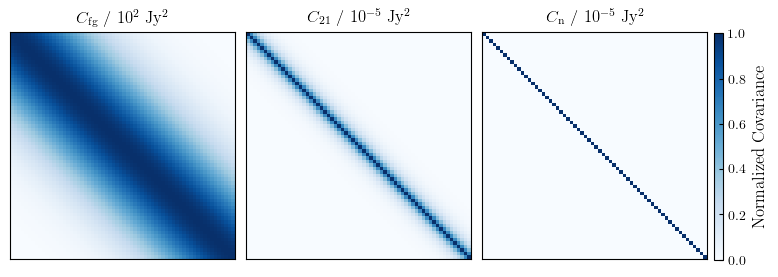
\includegraphics[scale=0.8]{imgs/data_covariance.png}
\caption{}
\label{fig:data_covariance}
\end{figure*}

\section{GPR Foreground Subtraction in the Quadratic Estimator Framework}
\label{sec:gprfs}

In this section we outline how GPR foreground subtraction can be incorporated into the quadratic estimator formalism.
We start by giving a brief review of quadratic estimators, and then demonstrate GPR-FS, or a GPR foreground subtracted quadratic estimator.
Principally, we show that this is closely related to the inverse covariance estimator outlined in \citet{Liu2011}.
We also discuss some variations to GPR-FS that allow for estimation of the foreground component (which is often useful for null testing and data quality management), in addition to handling the issue of missing data (e.g. due to RFI flags).
Lastly, most of the results of this section hinges on the assumption that the exact covariance of the data is known a priori.
Previous works have shown that one can either estimate the covariance from the data directly (T97, Seljak, Switzer?, Dillon2014), or one can adopt a fiducial covariance and iterate (Padmanabhan).
However, this is particularly tricky for EoR studies, where the EoR 21\,cm power spectrum is greatly unconstrained, and recent examples of empirically estimated covariances have led to signal loss \citep{Cheng2018}.
We discuss some of the potential pitfalls from this problem for detection of the EoR power spectrum at low $k$.

\subsection{Quadratic Estimators of the Power Spectrum}
\label{sec:qe}

The 21\,cm power spectrum is the square of the three dimensional Fourier transform of the temperature,
\begin{align}
\langle\widetilde{\T}(\boldsymbol{k})\widetilde{\T}^\ast(\boldsymbol{k}^\prime)\rangle = P(k)\delta(\boldsymbol{k}-\boldsymbol{k}^\prime),
\end{align}
where $\widetilde{\T}$ is the Fourier transformed temperature field, and $\delta$ is the Dirac-delta function.
Noting that the interferometric visibilities are simply the transverse Fourier transform of the sky (under the flat sky approximation), an estimate of the power spectrum can be made by directly Fourier transforming the visibilities across frequency into the delay domain $\tau$, known as the delay spectrum estimator \citep{Parsons2012a, Liu2014a}.
Due to the inherent chromaticity of the interferometer (i.e. it samples different spatial Fourier modes as a function of frequency), the visibility delay domain is not an exact mapping to the line-of-sight spatial Fourier domain, but for short baselines this is a fairly good approximation \citep{Parsons2012a}.
In this case, the power spectrum is defined as
\begin{align}
\label{eq:dspec}
P(k_\perp, k_\para) = \frac{X^2Y}{\Omega_pB}\langle\widetilde{V}(\boldsymbol{b}/\lambda, \tau)\widetilde{V}^\ast(\boldsymbol{b}/\lambda, \tau)\rangle,
\end{align}
where $X$ and $Y$ are scalars mapping angles on the sky to transverse cosmological distances and frequencies to line-of-sight cosmological distances, $\Omega_p$ is the integral of the primary beam and $B$ is the frequency bandwidth in the Fourier transform.
The cosmological wavevectors are related to the ``telescope units'' via
\begin{align}
\label{eq:kvecs}
k_\perp &= \frac{2\pi\tau}{X} \\
k_\para  &= \frac{2\pi}{Y}\frac{b}{\lambda},
\end{align}
where $X = c(1+z)^2\nu_{21}^{-1}H(z)^{-1}$, $Y=D(z)$, $\nu_{21}=1.420$ GHz, $H(z)$ is the Hubble parameter, $\lambda$ is the average observing wavelength, and $D(z)$ is the transverse comoving distance \citep{Parsons2014}.
In this work we adopt a $\Lambda$CDM cosmology with parameters derived from the Planck 2015 analysis \citep{Planck2016}, specifically $\Omega_\Lambda$=0.6844, $\Omega_b$=0.04911, $\Omega_c$=0.26442, and $H_0$=67.27 km/s/Mpc.

To be more statistically rigorous, we can cast the delay spectrum technique into the quadratic estimator framework \citep{Hamilton1997, Tegmark1997, Liu2014a}.
We start by approximating the continuous power spectrum as a piecewise function in sufficiently narrow bins in $k$.
The $\alpha$ bin's amplitude, $p_\alpha$, is referred to as its band power, and its reconstruction from the data is the ultimate goal of our estimator.
Fundamentally, we assume that the covariance of the data (in frequency space) can be related to the band powers as
\begin{align}
\label{eq:bandpowers}
\C = \N + \Cfg + \sum_\alpha p_\alpha \C_{,\alpha},
\end{align}
where $\N$ is our noise covariance, $\Cfg$ is our foreground covariance, $p_\alpha$ is our EoR power spectrum band powers, and $\C_{,\alpha} = \partial\C/\partial p_\alpha$ is the derivative of the covariance matrix with respect to the band powers.
A quadratic estimate of the band powers can be estimated from our data vectors as
\begin{align}
\label{eq:qe}
\hat{p}_\alpha = \d^\dagger\E_\alpha\d - b_\alpha,
\end{align}
where recall $\d$ is our data vector, $\hat{p}_\alpha$ is our estimate of the $\alpha$ band power, $\E$ is a family of matrices to-be-described, and $b_\alpha$ is an overall bias term.
Taking the expectation value of \autoref{eq:qe} and substituting in \autoref{eq:bandpowers}, we find that 
\begin{align}
\label{eq:window_funcs}
\hat{p}_\alpha = \sum_\beta\tr[\C_{,\beta}\E_\alpha]p_{\beta} + \tr[(\N + \Cfg)\E_\alpha] - b_\alpha.
\end{align}
\autoref{eq:window_funcs} tells us that for our estimator to be unbiased we set $b_\alpha = \tr[(\N+\Cfg)\E_\alpha]$.
Furthermore, it shows us that the estimated band powers $\hat{p}_\alpha$ are a linear combination of the true band powers $p_\alpha$ dictated by a transfer matrix, which we will denote as $\W$, commonly known as the \emph{window function}: $\hat{\p} = \W\p$.
The covariance of our band powers subject to the covariance of our input data can be written as
\begin{align}
\label{eq:qe_C}
\Sigma_{\alpha\beta} = \langle \hat{p}_\alpha\hat{p}_\beta\rangle - \langle \hat{p}_\alpha\rangle\langle \hat{p}_\beta\rangle = 2\tr[\C\E_\alpha\C\E_\beta].
\end{align}
The band powers, their window functions, and their covariance matrix completes our full statistical distribution of the EoR power spectrum \citep{Liu2014a}.

How do we actually compute these quantities?
The $\E_\alpha$ matrix can be decomposed as
\begin{align}
\label{eq:qe_E}
\E_\alpha = \frac{1}{2}\sum_\beta \M_{\alpha\beta} \R^\dagger \C_{,\beta} \R,
\end{align}
where $\M$ is a normalization matrix that ensures the estimated band powers are properly normalized, and $\R$ is an arbitrary data-weighting matrix, both of which the data analyst is free to choose subject only to the constraint that our band powers are properly normalized, or that $\sum_\beta\W_{\alpha\beta}=1$.
Here we also see the main role of $\C_{,\alpha}$ as a Fourier transform operator for the weighted data vectors on either side of it.
Given a choice of $\R$, we can compute the band power response matrix, defined as
\begin{align}
\label{eq:qe_response}
H_{\alpha\beta} = \frac{1}{2}\tr[\R^\dagger\C_{,\alpha}\R\C_{,\beta}],
\end{align}
which conveniently lets us re-express the window functions as $\W = \M \H$.

The most commonly adopted $\R$ matrix is $\R = \C^{-1}$, or the inverse data covariance matrix.
Given this weighting matrix and assuming a diagonal normalization matrix of $M_{\alpha\beta} = \delta^k_{\alpha\beta}\left(F_{\alpha\beta}\right)^{-1}$ where $\delta^k$ is the Kronecker delta, it can be shown that we recover the optimal, minimum variance estimator with the response matrix equal to the band power Fisher matrix, $\H = \F$, and the band power covariance equal to its inverse, $\boldsymbol{\Sigma} = \F^{-1}$ \citep{Hamilton1997a, Tegmark1997, Bond2000}.
Alternative choices of the normalization matrix lead to other desirable properties, such as $\M=\H^{-1}$ leading to window functions that are uncorrelated, and $\M=\H^{-1/2}$ leading to band power covariances that are uncorrelated.
While $\M=\H^{-1}$ normalization results in uncorrelated band powers, it does so at the expense of larger errorbars.
In this work, we therefore only use the minimum variance normalization (referred to as $\M\propto\I$) and the uncorrelated error normalization (referred to as $\M=\H^{-1/2}$).
In this work, regardless of the chosen normalization matrix, we refer to the optimal quadratic estimator as one that adopts $\R_{\rm OQE} = \C^{-1}$, which is also the ``inverse variance weighted foreground removal estimator'' described in \citet{Liu2011}.

To cast Gaussian process foreground subtraction into the quadratic estimator framework, we recognize that \autoref{eq:res} is simply a linear operation on the data vector, and can be equivalently expressed as
\begin{align}
\label{eq:gprfs}
\r = \d - \Exp[\f^\prime] = (\I - \Kfg[\Kfg + \Kto + \Kn]^{-1})\d  = \R_{\operatorname{GPR-FS}}\d.
\end{align}
A quadratic estimator that enacts a GPR foreground subtraction as part of its weighting matrix (referred to as GPR-FS) is therefore achieved by adopting the above $\R$ matrix.
Furthermore, variations about this technique are possible by dotting this matrix into other subsequent operators, such as additional, post-foreground removal weighting matrices.

\subsection{The Relationship Between GPR-FS and OQE}
\label{sec:gpr_oqe}

Here we show that the GPR foreground subtracted quadratic estimator (GPR-FS) is closely related to the optimal quadratic estimator, and is in fact identical to OQE when dotting the former with an additional inverse covariance weighting matrix.
For the time being, we will assume we know the true covariance of the data and will adopt terms like $\Cfg$ instead of $\Kfg$ in our equations.
We can prove the equivalence of these two estimators by using the Woodbury matrix identity, which states that for an invertible matrix $\A$ and for a matrix $\B$ that can be decomposed as $\B = \U\S\V^\dagger$,
\begin{align}
[\A + \U\S\V^\dagger]^{-1} = \A^{-1} - \A^{-1}\U[\S^{-1} + \V^\dagger\A^{-1}\U]^{-1}\V^\dagger\A^{-1}.
\end{align}
In our case, both $\A$ and $\B$ are taken to be Hermitian covariance matrices, implying that $\U$ and $\V$ are unitary matrices subject to $\U\V^\dagger = \I$, with $\S$ being a diagonal eigenvalue matrix.
Re-arranging, we find that
\begin{align}
[\A + \U\S\V^\dagger]^{-1} &= \A^{-1}(\I - \U[\A\U\S^{-1} + \U]^{-1}) \nonumber \\ 
&=\A^{-1}(\I - \U\S\V^\dagger[\A + \U\S\V^\dagger]^{-1})
\end{align}
where in the first equality we pulled $\V^\dagger\A^{-1}$ into the bracketed inverse and used the fact that $[\V^\dagger]^{-1} = \U$, and in the second equality formed the quantity $\U = \U\S\V^\dagger[\S\V^\dagger]^{-1}$ and pulled part of it into the bracketed inverse.
Substituting in $\A = \Cn + \Cto$ and $\B = \Cfg$, we get that
\begin{align}
[\Cn + \Cto + \Cfg]^{-1} &= [\Cn + \Cto]^{-1}(\I - \Cfg[\Cn + \Cto +  \Cfg]^{-1}) \nonumber \\
\R_{\rm OQE} &= [\Cn + \Cto]^{-1}\R_{\operatorname{GPR-FS}}
\end{align}
which tells us that a GPR-FS weighting matrix dotted with an additional inverse noise and EoR covariance weighting matrix is equal to the inverse of the full data covariance matrix.
Given that the statistical properties of a quadratic estimator are uniquely defined by the choice of $\R$ matrix (holding our choice of $\C_{,\alpha}$ constant), we conclude that the optimal quadratic estimator and the inverse variance weighted GPR-FS estimator are actually identical power spectrum estimators.
This is an interesting and non-intuitive result that helps us understand the properties of both of these methods.
First, we see that the inverse covariance foreground separation method of \citet{Liu2011}--the OQE of the 21\,cm signal in the presence of foregrounds--can in fact be re-cast as a Gaussian Process, with \autoref{eq:fg_conditional} yielding its constrained foreground estimate.
Second, we see that the window function and band power covariance matrices for the GPR foreground subtraction technique can be easily derived, and are in fact similar to those for the optimal estimator.

Lastly, we note that GPR foreground subtraction need not only apply to foregrounds.
By simply substituting $\Kfg$ with the sum of any number of covariances describing terms in the data that we would like to subtract, we can construct a GPR-based signal separation estimator that is functionally equivalent to what the optimal quadratic estimator would achieve.

\begin{figure*}
\centering
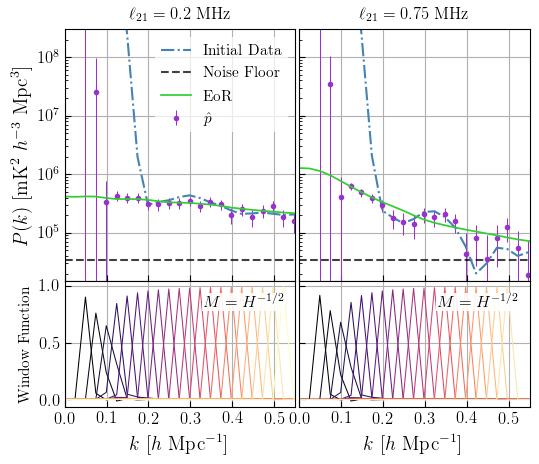
\includegraphics[scale=0.6]{imgs/gpr_window_low_noise_M_F12}
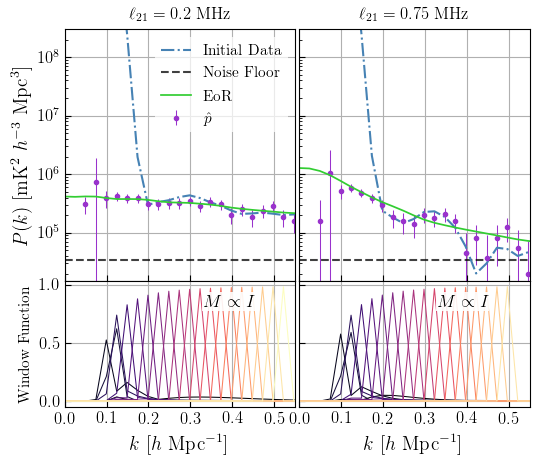
\includegraphics[scale=0.6]{imgs/gpr_window_low_noise_M_I}
\caption{Mock GPR foreground separation for two different EoR models ($\ellto$ = 0.25 \& 0.75 MHz) and two different normalization schemes, $M=F^{-1/2}$ (left) and $M\propto I$ (right), in a \emph{low noise scenario} where we get a nominal 10$\sigma$ detection at $k\sim0.2\ h\ {\rm Mpc}^{-1}$.
We show the full data consisting of foregrounds, EoR, and noise (blue dashed), the integrated noise floor of the data (black dashed), the intrinsic EoR component (green solid), and the GPR-FS quadratic estimates (purple dots) after 1000 (independent) incohorent averages.
The error bars on the band powers are their 1$\sigma$ uncertainty ($\sqrt{\Sigma_{\alpha\alpha}}$).
For both EoR models and under both normalization schemes, GPR-FS returns unbiased band power estimates at large $k$ modes.
However, we see that without band power decorrelation (i.e. in the $\M\propto\I$ regime), GPR-FS fails to return statistically independent estimates of the band powers for $k<0.1\ h\ {\rm Mpc}^{-1}$, evidenced by the lack of power in the window functions (lower right).
Although the decorrelated band power window functions demonstrate they can make largely statistically independent measurements at these low $k$ modes, their associated uncertainty is dramatically inflated.
TODO: fix P(k) units.
}
\label{fig:gpr_window_low_noise}
\end{figure*}

\begin{figure*}
\centering
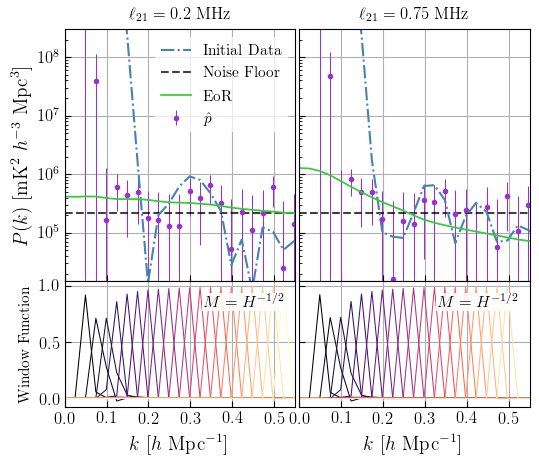
\includegraphics[scale=0.6]{imgs/gpr_window_med_noise_M_F12}
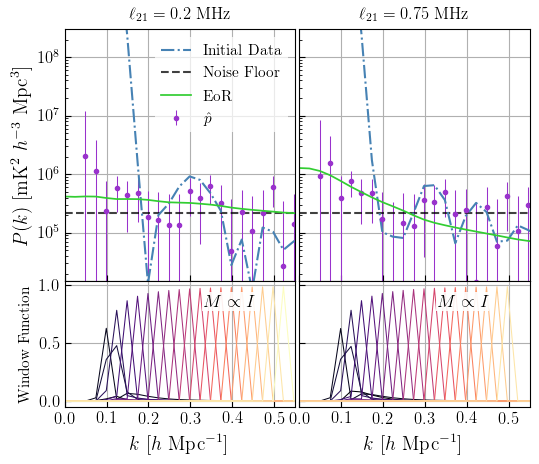
\includegraphics[scale=0.6]{imgs/gpr_window_med_noise_M_I}
\caption{The same as \autoref{fig:gpr_window_low_noise} but in a \emph{moderate noise scenario}, where the averaged noise floor roughly meets the EoR signal at $k\sim0.2\ h\ {\rm Mpc}^{-1}$.
In this scenario the window functions are slightly better behaved; however, we still see that GPR-FS with $\M\propto\I$ normalization is unable to probe the very low $k$ modes of the power spectrum.}
\label{fig:gpr_window_med_noise}
\end{figure*}

\subsection{Mapping the Window Functions}
\label{sec:gpr_windows}

One of the blessings of incorporating GPR modeling into the quadratic estimator formalism is the ability to compute the band power window functions.
The window functions tell us how the intrinsic band powers map into our measured band powers.
In a sense, they represent the true $k$ mode that our band powers are centered on and the width of the band power bin (i.e. the horizontal error bar): the $k$ bin our band powers are actually sensitive to may not be the naive $k$ bin we would expect from a simple Fourier transform.
To demonstrate an idealized case of GPR-FS and to map its window functions, we generate mock visibility data from the foreground, EoR, and noise covariances described in \autoref{sec:gpr}.
Again, we assume that we know the true covariance of the data a priori (which will be relaxed later).
\autoref{fig:data_covariance} shows the covariances of our three data terms.
We simulate a single visibility waterfall from 120 -- 140 MHz with 64 frequency channels by drawing from a mean--zero complex Gaussian distribution with the above covariances and sum the three terms together.
We repeat this 1000 times (independently for each time) and stack them to construct a data vector $\d$ of shape $(N_{\rm freqs}, N_{\rm times}) = (64, 1000)$.


We can also show this result holds numerically.
To do this we construct a toy model simulation (not the sky model based simulations discussed in other parts of this work) that is simply a series of random draww from a known covariance.
We adopt the same foreground, noise and EoR covariances described in \autoref{sec:gpr} with their kernel hyperparameters set as $\{\sigmafg^2, \ellfg, \sigmato^2, \ellto, \sigman^2\} = \{ {\rm Jy}^2, {\rm MHz}, {\rm Jy}^2, {\rm MHz}, {\rm Jy}^2\}$.
First, we draw randomly from these covariances independently and sum their results, and then repeat this 1000 times to make an ensemble of toy model simulations.
For each simulation we form four products: 1) the inverse covariance weighted quadratic estimate with $\R=[\Cfg + \Cn]^{-1}$, 2) the GP foreground subtracted quadratic estimate with $\R=\I - \Cfg[\Cfg + \Cn]^{-1}$, 3) the uniformly weighted quadratic estimate with $\R = \I$, and 4) the uniformly weighted quadratic estimate of only the EoR component of the data.
In we show the power spectra and their associated uncertainties (errorbars are $\sqrt{\Sigma_{\alpha\alpha}}$).
The points in the left and right panels show the Gaussian Process subtracted quadratic estimate and inverse covariance weighted quadratic estimate, respectively, while the green line shows the uniformly weighted simulation (showing the intrinsic amplitude of the un-subtracted foregrounds at low $\kpara$) and the red line shows the uniformly weighted EoR component (showing the true EoR bandpowers).
In both cases, we see that foreground subtraction is able to remove the bright foregrounds at low $|\kpara|$ down to EoR amplitudes.
While the foreground-subtracted bandpowers show deviation from the true EoR bandpowers at low $|\kpara|$ (comparing the red line to points), the uncertainties on the estimated bandpowers is also boosted at these modes, such that the uncertainties on the estimated bandpowers encompass the true bandpowers.



\begin{figure}
\centering
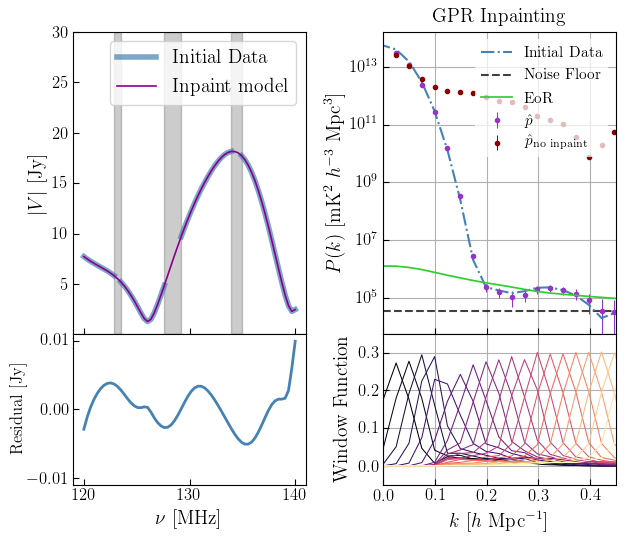
\includegraphics[scale=0.5]{imgs/gpr_low_noise_inpainting}
\caption{GPR inpainting applied to the mock dataset from above. {\bfseries Left}: We show the initial data (blue) with flags applied (shaded) and the inpaint model (purple), which is only summed with the data in the flagged regions. The residual between the inpaint model and the initial data is also plotted (bottom). {\bfseries Right}: We plot the inpainted power spectrum compared to the original data (purple), EoR signal (green solid) and the noise floor (black dashed), along with the non-inpainted band powers (red). All power spectra are normalized with $\M\propto\I$ convention. We also show the inpainted window functions (bottom). }
\label{fig:gpr_low_noise_inpainting}
\end{figure}


\subsection{Wideband GPR-FS}
\label{sec:wideband_gpr}

In this section we propose a method for modeling and removing foregrounds across a wide frequency bandwidth (thus achieving finer delay resolution in Fourier space), while simultaneously taking narrow-band power spectra.
The advantage to this, as opposed to modeling the foregrounds over the same narrower spectral window used for estimating the power spectrum, is the improved behavior of the resultant window functions, driven by the finer delay resolution achievable when modeling across a wider bandwidth \citep{Parsons2014}.
This comes at the cost of increased computational complexity (recall GP's naively scale as $N^3$) as well as an increased data model complexity.
Previous works applying GPR foreground subtraction have made simplifying assumptions driven in part by the adoption of a narrow bandwidth--namely that the foreground and noise covariance amplitude is constant over the band.
Over wide bandwidths, this assumptions breaks down, as both the foreground and noise variance increase significantly with decreasing frequency: in practice, an amplitude power law model would need to be added to the foreground and noise covariances.
In this section we do not actually do this, as this is merely a proposal for how one can setup a wideband GPR-FS matrix, and is meant to demonstrate the improved performance over a narrowband GPR-FS.

A wideband GPR-FS is simply a larger, rectangular $\R$ matrix of shape $N_{\rm spw\ freqs}\times N_{\rm freqs}$, where $N_{\rm spw\ freqs}$ is the number of frequency channels in the narrowband spectral window used for power spectrum analysis, and $N_{\rm freqs}$ is the number of frequencies across the wider bandwidth used for GPR modeling.
To demonstrate this, we use the same 




\subsection{Inpainting Missing Data}
\label{sec:inpainting}
Often when working with real instruments we must excise or flag data due to poor quality.
This can motivated by detector or instrument failures or by contamination of certain parts of the data, for example due to radio frequency interference.
Intensity mapped power spectra are particularly sensitive to missing data along the frequency axis, as a Fourier transform of discontinuous features will cause ringing of bright Fourier modes (such as foregrounds) to other modes thus contaminating them.
Solutions to this problem have been to remove as much of the foregrounds as possible in the frequency domain (see \citet{Ewall-Wice2020} for an example of this), or to deconvolve the effect of missing data in Fourier space.
Nevertheless, for realistic foreground subtraction techniques we often find residual systematic features that are stronger than the EoR signal in certain parts of Fourier space.
In theory band power decorrelation (e.g. setting $\M=\F^{-1}$) can help with this, but can often in practice be limited by numerical precision (\nsk{this is just my intuition having trouble doing so in practice}): inpainting can help prevent these features from contaminating other modes in the first place.
In practice we are less concerned about the EoR signal ringing against itself in Fourier space, as most theoretical models predict fairly flat features in $P(k)$, but in general this is still a concern, and eliminating the ringing of the EoR signal can help to prevent unnecessary correlation between nearby band powers of high SNR detections.
Furthermore, another reason for wanting to inpaint the data is because we often want to make power spectra of the foreground component, as this is a useful metric for assessing data quality and performing jacknife and null tests.

In general, the problem of reconstructing a signal from incompletely sampled data is known as compressed sensing.
An example of a well-known radio astronomy technique for solving this problem is the Hogbom CLEAN algorithm and its derivatives \citep{Hogbom1974}.
A 1D variation of this algorithm applied along the frequency axis of radio visibilities has been extensively used in PAPER and HERA data analyses \citep{Parsons2009, Ali2015, Kerrigan2018, Kern2020a}.
Recently, \citet{Trott2020} explored how GPR inpainting (aka `kriging') can be used to partially mitigate the effect of regularly contaminated frequency bins in MWA data.
In addition, \citet{Ewall-Wice2020} recently presented a linear filter that uses a delay-space maximum likelihood method for inpainting missing data.
Inpainting also has a long history in CMB analyses, applied to both $C_\ell$ estimation () and map making ().
Here we demonstrate how data inpainting can be seamlessly incorporated into the GPR-FS quadratic estimator, thereby including its effect into the full statistical description of the band power window function and covariance matrix.

Recall \autoref{eq:gp_conditional} gives the distribution of the desired latent variable conditioned on the data.
For the purposes of foreground subtraction, the desired latent variable was assumed to be the foreground component sampled at the same frequencies as the data (\autoref{eq:fg_conditional}).
For the purpose of inpainting we can relax some of these assumptions.
First, inpainting should only impact the data voxels with missing data, and should not alter otherwise cleanly sampled data.
Therefore, the output of the GP model should be summed with the data vector only at the flagged frequency bins.
Furthermore, we do not want the GP conditioned on the missing data, as it is not part of the statistical distribution we are trying to model.
We can handle this by either giving those frequency bins an infinite noise variance (thus in practice eliminating their contribution to the data model), or we can simply truncate them from the data vector $\d$, as the GP need not sample the data at regularly spaced intervals.
To be consistent with $\nu$ representing the native data frequencies and the input frequencies to the GP, we will adopt the former convention.
Second, we may want to inpaint multiple components of the data, not just the foreground signal.
To capture this, we define $\dip$ as the latent variable to-be-inpainted in frequency space, and $\Kip$ as our model for its covariance.


This leads us to construct a generic Gaussian process data model matrix (GPR-DM)
\begin{align}
\label{eq:gpfm}
\R_{\operatorname{GPR-DM}} = \Kip[\Kfg + \Kto + \Kn]^{-1},
\end{align}
which gives us the GPR estimate of our latent variable at all data frequencies.
We can combine this with the appropriate weighting matrices to construct an inpainting matrix,
\begin{align}
\label{eq:gprip}
\R_{\operatorname{GPR-IP}} = \W_{\rm uf} + \W_{\rm f} \R_{\operatorname{GPR-DM}}
\end{align}
where $\W_{\rm f}$ is a diagonal weight matrix that is zero at unflagged frequencies and one at flagged frequencies, and $\W_{\rm uf}$ is a diagonal weight matrix that is zero at flagged frequencies and one at unflagged frequencies.
When forming power spectra of data with a large dynamic range between Fourier modes, it is often beneficial to apply a tapering function that smoothly connects that data to zero at the band edges (also known as apodization), which limits the Fourier space ringing induced by the fact that our data are finitely sampled.
We can do this adopting $\T\R_{\operatorname{GPR-IP}}$ as our weighting matrix, where $\T$ is a diagonal matrix with a tapering function applied to its diagonal.
A commonly adopted taper--and the one we adopt here--is the Blackman-Harris function, which returns 5 orders of magnitude in sidelobe suppression \citep{Blackman1958}.

In \autoref{fig:gpr_low_noise_inpainting}, we show an example of this estimator applied to the same data products discussed above.
The left panel shows the foreground model constructed from $\R_{\operatorname{GPR-DM}}$ (purple) compared to the initial data, along with the flagged regions (shaded).
The right panels shows the estimated power spectrum with and without inpainting (with $\M\propto\I$ normalization) along with the inpainted band power window functions.
Inpainting helps us recover accurate estimates of the foreground power over spectral windows with missing data, which can be useful for data quality management and null testing of data analysis pipelines \citep{Kolopanis2019}.


\subsection{The Impact of Imperfect Covariance Models}
\label{sec:cov_models}

The results of this section have thus far made the generally unrealistic assumption that we know the true covariance of the data a priori.
In principle this is reconcilable, as we can either estimate the covariance from the data, or adopt a prior covariance, produce power spectra, update the covariance, and iterate \citep{Bunn1995, Tegmark, Padmanabhan2001}.
Empirical covariance estimators have both been studied and used in 21\,cm analyses \citep{Dillon2014, Ali2015, Switzer, Eastwood, Masui}, but have also been a point of contention in the literature, as certain aspects of how one derives and regularizes an empirical covariance have been shown to be susceptible to signal loss \citep{Cheng2018}.
In particular, signal loss was shown to occur when one's covariance is too finely tuned to the dataset at hand: in other words, if the covariance is overfit.
However, another source of concern for foreground subtraction techniques is in the subtraction of the \emph{foreground bias}, $b^{\rm fg}_\alpha = \tr[\Cfg\E_\alpha]$.

In this section, we focus on the impact of 


\subsection{Reconciling the Bias Correction of M20}
\label{sec:bias_correction}

In \citetalias{Mertens2020} Sec. 3.3.2 it is postulated that the inferred variance of the residual vector after GPR foreground subtraction is a biased estimate, and can be corrected to be unbiased by summing its variance with the variance of the GP foreground estimate (\autoref{eq:fg_cov_conditional}).
At face value, this seems similar to a power spectrum normalization step, either in the mapping of $q$ to $p$ via the $\M$ matrix or in the subtraction of the $b_\alpha$ term in the QE formalism.
We claim, however, that this is in fact not the same as a proper power spectrum normalization or bias subtraction, and that its statistical implication for the resultant band powers warrants further scrutiny.

To summarize \citetalias{Mertens2020}, the covariance of the residual vector can be shown to be
\begin{align}
\label{eq:res_covariance}
\langle\r\r^\dagger\rangle = \R_{\operatorname{GPR-FS}}\langle\d\d^\dagger\rangle\R_{\operatorname{GPR-FS}}^\dagger
\end{align}


The band power bias correction is motivated by the fact that the covariance of the foreground residual (\autoref{eq:gp_conditional}) is found to be equal to the covariance of the residual terms minus the covariance of the foreground estimate.
This is derived under the assumption that $\langle \d \d^\dagger\rangle = \Kfg + \Kto + \Kn$, or that the ensemble average of the data is equal to the adopted covariance model.
Note that this is a much different assumption than that found in the quadratic estimator




%%%%%%%%%%%%%%%%%%%%%%%%%%%%%%%%%%%%%%%%%%
%%%%%%%%%%%%%%%%% Simulation %%%%%%%%%%%%%%%%%%%
%%%%%%%%%%%%%%%%%%%%%%%%%%%%%%%%%%%%%%%%%%
\section{Simulating HERA Observations}
\label{sec:sims}

We use the \texttt{healvis}\footnote{healvis} simulation software \citep{Lanman2019} to generate realistic interferometric visibilities.
\texttt{healvis} represents the sky, primary beam and fringe pattern (the three main components of \autoref{eq:me}) as HEALpix maps \citep{Gorski}, and approximates the sky integral with a discrete sum.
\autoref{Lanman2019} showed that, at low frequencies ($\nu\sim150$ MHz) and for intermediate baseline lengths of $|b| < 150$ m, \texttt{healvis} converges to a stable result with a HEALpix maps with NSIDE = 256 resolution.
In this section we discuss the various components of our simulation.
The simulations are specific to HERA in the sense that the baseline $uvw$ coordinates are adopted from a fiducial HERA layout and in that the adopted primary beam model is an airy disk representative of HERA's 14-meter dishes; however, this is easily extensible and we could readily use this framework to produce simulations more specific to the MWA or LOFAR, for example.
We do not expect the fundamental results of this work--in other words, the overall performance of GP modeling on simulated data--to be strongly dependent on the telescope model, as the statistics of the underlying sky signals are not significantly changed.\footnote{The one exception to this is the usage of particularly short baselines in this work, $\lambda \sim 20$, whereas similar works on LOFAR use $\lambda\sim XX$, which can have significant ramifications of the statistics of the observed 21\,cm and foreground signal in the visibilities.}
\autoref{tab:simulation} details the various components of our data simulations.
The angle and frequency dependence of the Airy disk primary beam is the result of a uniformly-illuminated circular aperture, written as
\begin{align}
A(\theta, \nu) = \frac{\nu}{c\pi D\sin\theta}J_1\left(\frac{c\pi D\sin\theta}{\nu}\right),
\end{align}
where $\theta$ is the angle in radians away from the pointing center, $D=14$ meters is the dish diameter, and $J_1$ is the first-order Bessel function of the first kind.
\autoref{fig:ant_array} shows the HERA array layout used in our simulations.
We simulate the 10 shortest unique baselines (including the auto-correlation), which consists of all baselines between numbered antennas paired with antenna 0.

\begin{table}
\centering
\begin{tabular}{l l} 
\hline
\hline
{\bfseries Telescope Parameters} \\
Array layout & HERA Hexagonal \\
Number of simulated baselines & 10 \\
Min. baseline length & 14.6 m  \\
Max. baseline length & 58.4 m \\
Observation type & drift-scan \\
Primary beam & 14-meter airy disk \\
Frequency band & 120 -- 140 MHz \\
Channel width & 156.25 kHz \\
Observation LST & 1.0 hour \\
Number of integrations & 1 \\

\hline
{\bfseries Signal Parameters} \\
Diffuse Foreground Term & 2008 Global Sky Model \\
Point Source Foreground Term & MWA GLEAM Catalogue \\
EoR Term & \texttt{21cmFAST} lightcone \\
HEALPix Map NSIDE & 256 \\
Sky Noise Term & GSM total power with HERA $\Omega_p$ \\
Receiver Noise Term & 100 Kelvin \\
Contaminants & Gain errors and RFI \\
\hline
\hline
\end{tabular}
\caption{Data simulation signal terms and parameters for this work. More details in \autoref{sec:sim_app}.}
\label{tab:simulation}
\end{table}

\begin{figure}
\centering
\includegraphics[scale=0.6]{imgs/ant_array}
\caption{HERA array layout used for our simulations. We simulate the 10 shortest unique baseline types formed between all numbered antennas paired with antenna 0.}
\label{fig:ant_array}
\end{figure}

\subsection{Foregrounds}
Diffuse foreground emission is modeled using the Global Sky Model \citep[GSM;][]{Oliveira2008}.
Point source model comes from the GLEAM survey.

\begin{figure}
\centering
\includegraphics[scale=0.5]{imgs/sim_vis.png}
\caption{Simulated data products in frequency space and in Fourier space for a 30-meter baseline. Diffuse foregrounds (upper-left, green) are smoothly varying but have spectral structure imparted by the chromaticity of the instrument. EoR (lower-left, blue) is highly spectrally variant, and thermal noise (upper-right, grey) has uncorrelated power on all scales. The thermal noise amplitude shown here is for an instantaneous 10.7 second HERA snapshot observation, but is lowered when running GPR to simuate longer integration times. The diffuse foreground component alone is roughly $10^10$ greater in power than the EoR (lower-right).}
\label{fig:sim_vis}
\end{figure}

\subsubsection{A Note on ``Mode Mixing''}
Foregrounds that are spectrally smooth occupy low line-of-sight (LoS) spatial Fourier modes ($k_\para$).
Certain effects from the instrument and from the environment, however, can cause these modes to leak-out to higher $k_\para$.
In general, anything that creates spectral structure, (e.g. unflagged RFI, primary beam variations, residual gain errors, etc), will create this leakage.
However, another way this leakage is created is simply due to the chromaticity of the instrument, as discussed in \autoref{sec:rime}.
This effect is not really an imperfection of the instrument because even an idealized interferometer (e.g. in the absence of imperfect calibration, ionosphere, PB variations) defined by \autoref{eq:rime} will see this effect.
Traditionally, it is this latter effect that has been called ``mode mixing'' in the literature \citep{Datta, Morales}, not the former, non-idealized effects like RFI and PB variations.
In this work we will stick to this convention.
Therefore, mode mixing terms are automatically included in our foreground simulation via \autoref{eq:rime}, and do not actually need to be simulated as a post-processing step as is done in \citet{M19}.
However, we do simulate certain non-idealized effects like calibration errors that are in practice ubiquitous in real data.


\subsection{21\,cm Signal}
Our 21\,cm cosmological signal simulations start with $\delta T_b$ box output from the \texttt{21cmFAST} semi-numerical simulation \citep{Mesinger2011}.
This simulation uses 1st order Lagrangian perturbation theory to evolve the dark matter density field starting from initial conditions at $z=300$ down to EoR redshifts, and then uses approximate physics to evaluate the HI ionization field using an excursion set approach and a combination of semi-analytic parameters that govern the ionizing photon production efficiency of star forming galaxies \citep{Furlanetto}.
We further assume a saturated spin temperature that is appropriate only in the limit of a strongly heated IGM.
For the redshifts we are concerned with ($6 < z < 10$) this is a fairly good approximation, although this begins to break down towards the high redshift end, and is also not appropriate in scenarios of late or weak IGM heating \citep{Greig, Mirocha}, which have not been ruled out by observations.
Our use of approximate physics for the 21\,cm component is justified for this work because we are concerned only with generating a statistically plausible realization of the 21\,cm field.
The primary concern of this work is whether we can recover that signal, regardless of how it is generated, with the techniques described.

In running \texttt{21cmFAST}, we use the default parameterization, $\zeta=$, $T_{\rm vir}=$, $R_{\rm mfp}=$.
We use a box with a side length $L=X$ Mpc with a grid resolution of X$^3$ to sample and evolve the dark matter initial conditions, which are then downsampled to X$^3$ to calculate the $\delta T_b$ field, yielding a final voxel resolution of X Mpc$^3$.
For each observing frequency and HI emitter redshift, the $\delta T_b$ box output is then stacked in 3D real space and then sampled within a thin spherical annulus at the appropriate comoving distance to create large-scale HEALpix maps using \texttt{cosmotile}\footnote{cosmotile} package \citep{Kitisiwit}.
These maps are then fed into the normal \texttt{healvis} simulation framework.



\subsection{Contaminants}
\label{sec:contaminants}

\subsubsection{Residual Direction Independent Gain Errors}
Even after instrumental calibration, there is likely to be residual gain errors that have temporal and spectral components.
These will cause leakage of the foregrounds out to higher $\kpara$ modes.
We simulate residual DI gain errors that are smoothly varying in time with a 6 hour timescale, with decaying spectral structure out to 500 ns.
These fiducial choices are motivated by HERA calibration studies \citep{Kern2020a, Kern2020b}.


\subsubsection{Residual Direction Dependent Gain Errors}


\subsubsection{Cross-Coupling}


\subsubsection{Cable Reflections}
We do not simulate cable reflections in this work, although they are a common systematic for radio surveys and have been observed in almost all leading 21\,cm experiments.
Instead, we assume that cable reflections have been mostly calibrated out by calibration procedures, and the residual


\subsubsection{Radio Frequency Interference}


residual phase and amplitude gains, RFI, crosstalk?

realistic simulation and statistical simulation from the kernel (as is done in M19).


\subsection{Noise}
Thermal noise in the visibilities is drawn from a complex normal distribution with a standard deviation proportional to the system temperature $T_{\rm sys}$.
For HERA Phase I, this has been shown to be roughly 300 K for $\nu\sim150$ MHz.


\subsection{Unexplored Effects} 
Ionosphere, polarization leakage, etc.


%%%%%%%%%%%%%%%%%%%%%%%%%%%%%%%%%%%%%%%%%%
%%%%%%%%%%%%%% Simulated HERA Trials %%%%%%%%%%%%%%%%
%%%%%%%%%%%%%%%%%%%%%%%%%%%%%%%%%%%%%%%%%%
\section{Mock Foreground Subtraction for HERA}
\label{sec:hera_gprfs}
In this section we apply GPR-FS to the simulated HERA observations discussed above.


The seminal conclusion of \citetalias{Mertens2018} is that by developing a covariant description of each of the signal terms in the data, $\{\f, \e, \n\}$, one can model the foreground term in a way that allows for a clean subtraction of the 21\,cm signal from the other components in the data.
In particular, they emphasize that this can even be done even in the limit that the 21\,cm signal is appreciably below the thermal noise floor (i.e. $\sigma_{N} > \sigma_{21}$), which they show by taking their residual power spectrum and subtracting the noise bias \emph{inferred from the same noise realization used in their simulations} to reveal a non-zero fluctuations that is visually consistent with their input 21\,cm power spectrum (their Figure 4).
However, this result does not support their original claim because this kind of operation can never be realized in practice: one can never estimate the noise power to better precision than the underlying noise floor of the data.
In other words, we are never handed the \emph{actual} noise bias found in our data, and therefore must estimate its amplitude from the data itself, which fluctuates at the level of the thermal noise.
To answer the question we think they are trying to get at--which is if GPR modeling performed on noisy data can leave intact a weaker 21\,cm signal--one should run GPR on many independent realizations of noisy data and then coherently integrate them to reduce the noise floor.
This is important because the former approach (removing the exact noise fluctuations used in the simulation) may hide the fact that while GP modeling may leave the \emph{variance} of the 21\,cm signal in the data, it may not leave intact its underlying mean function.
Forcing one to coherently integrate an ensemble collection of residual vectors would reveal this failure mode, as the 21\,cm residuals would quickly de-correlate and show readily observable signal loss compared to the input simulated signal.

\citetalias{Mertens2018} model the EoR term with a Matern kernel with $\nu=1/2$, and model the foreground term with the sum of an intrinsic term and a mixture term, using a Matern kernel with $\nu=5/2$ and $\nu=3/2$, respectively.
Both the overall variance of the kernels and their length scales are left as free hyperparameters to be constrained by the data, and the choice of $\nu$ for the Matern kernels is motivated by a model selection test using the marginal likelihood (or Bayesian evidence).
Noise is modeled as homoscedastic\footnote{in principle, noise is generally heterscedastic and various both as a function of LST and frequency, but over narrow time and frequency ranges homoscedasticity is not a bad approximation}, and is fixed at the measured noise level of the data.

%While the mixture kernel is intended to account for mode mixing induced by instrument chromaticity and other contaminants, modeling it as a separate and uncorrelated term is not totally appropriate as it is simply a convolution of the intrinsic foregrounds with a chromaticity kernel, and is therefore likely to be correlated with the intrinsic sky term in the data.




%This latter point is reinforced by the fact that, as we will see, GP modeling shows significant EoR-to-FG power leakage at low $k$ modes that must be accounted for by an overall scaling factor to even make an unbiased measurement of the EoR.

In our GPR runs below, we optimize the GP kernel and evaluate \autoref{eq:fg_conditional} on each simulated baseline independently.
This is technically different than what \citetalias{Mertens2018} did, which is to optimize the kernel for a set of baselines simultaneously for computational savings.
However, our approach is likely to lead to more accurate results, as different baselines will have slightly different underlying data covariances \citep{Ghosh2020}.
Furthermore, we train the GP on the real and imaginary component of the visibility simultaneously (i.e. as separate features of the same underlying data vector).
When optimizing the kernel over its hyperparameters, we hold the noise kernel fixed at its value \emph{estimated} from the data (we do not set it to the exact pre-defined value).


\begin{table}
\centering
\begin{tabular}{l c c} 
 \hline
 \hline
 Hyperparameter & Uniform Prior Bounds & Posterior Bounds \\
 \hline
 {\bfseries High SNR Regime} \\
 $\sigma_{\rm n}$ [Jy] & 1.14$\times10^{-3}$ & -- \\[.1em]
 $\sigma_{\rm fg}$ [Jy] & 0, $10^3$ & $34.2 \pm 7.0$  \\
 $\ell_{\rm fg}$ [MHz] & 2, 50 & $4.33 \pm 0.13$ \\
 $\sigma_{\rm 21}$ [Jy] & $10^{-5}$, 1 & $(2.38\pm0.12)\times10^{-3}$ \\
 $\ell_{\rm 21}$ [MHz] & $10^{-5}$, 3 & $0.10 \pm 0.02$ \\
  \hline
{\bfseries Low SNR Regime} \\
 $\sigma_{\rm n}$ [Jy] & 1.66$\times10^{-4}$ & -- \\
 $\sigma_{\rm fg}$ [Jy] & 0, $10^3$ & --\\
 $\ell_{\rm fg}$ [MHz] & 2, 50 & --\\
 $\sigma_{\rm 21}$ [Jy] & $10^{-5}$, 1 & --\\
 $\ell_{\rm 21}$ [MHz] & $10^{-5}$, 3 & --\\
 \hline
 \hline
\end{tabular}
\caption{GP hyperparameter selections for \autoref{sec:M18}. All priors (except for $\sigman$, which is fixed) are uniform.}
\label{tab:hp_priors}
\end{table}


\begin{figure}
\centering
\includegraphics[scale=0.4]{imgs/gp_fg_fit}
\caption{Foreground model fit (dashed-green) to the underlying visibility data (black) in the high SNR regime. The residual vector is shown (red) next to the underlying EoR signal (blue), showing a good but not perfect match.}
\label{fig:gp_fg_fit}
\end{figure}


\subsection{High SNR Regime}
\label{sec:high_snr}

\begin{figure*}
\centering
\includegraphics[scale=0.5]{imgs/high_snr_gpr.png}
\includegraphics[scale=0.45]{imgs/high_snr_hp_posterior.png}
\caption{Left: Power spectra of the data (black), foreground model (dashed green), intrinsic EoR component (blue), residual (red), and statistical noise floor (dashed grey) in the high SNR regime. Right: Hyperparameter posterior distributions for a 30-meter baseline. The preference for a $\sigmato/\sigman$ > 1 shows a clear detection of the 21\,cm signal by the covariance kernel. Contours show the 68\% and 95\% confidence intervals.}
\label{fig:high_snr}
\end{figure*}

\begin{figure*}
\centering
\includegraphics[scale=0.5]{imgs/low_snr_gpr.png}
\includegraphics[scale=0.45]{imgs/low_snr_hp_posterior.png}
\caption{Left: Power spectra of the data (black), foreground model (dashed green), intrinsic EoR component (blue), residual (red), and statistical noise floor (dashed grey) in the low SNR regime. Right: Hyperparameter posterior distributions for a 30-meter baseline. The posterior on $\sigmato$ shows a detection (i.e. it is not consistent with $\sigmato=0$), however, the strength of the detection on both $\sigmato$ and $\ellto$ is considerably weaker than in the high SNR limit. Contours show the 68\% and 95\% confidence intervals.}
\label{fig:low_snr}
\end{figure*}

We start by assuming that our data have been integrated enough such that the per-visibility thermal noise is below the EoR signal ($\sigma_n = 0.5 \sigma_{21}$).
This is a highly idealized assumption, and is equivalent to roughly three full years of uninterrupted integration (180 observing days per year) for one of HERA's short redundant baseline types for the full array (350 elements).
This is a useful benchmark because it represents a best-case scenario, where thermal noise is not a major limiting factor above the EoR amplitude.

We regress for the kernel hyperparameters (\autoref{tab:hp_priors}), which fall well within the bounds of the hyperparameter priors.
\autoref{fig:gp_fg_fit} shows the MAP foreground model (dashed-green) compared to the underlying data.
We see that the foreground model is a very good fit, with the residual vector highly comparable, but not identical, to the underlying EoR signal in the data.
To understand the impact foreground removal has on the power spectrum, we form cross power spectra of the data, the residual, and the foreground model and plot them in \autoref{fig:high_snr}.
Again, we see that the foreground model is a good fit to the foreground structure in the data, however, we see that within the wedge the residual is inconsistent with the EoR or even the thermal noise.
For $k_\para < 0.2$ Mpc$^{-1}$, we find that the foreground model over-subtracted the signal and removed both intrinsic EoR and noise structure that was not supposed to be modeled by the foreground kernel.
In other words, while the RBF kernel does an excellent job modeling the smooth foreground signal to high dynamic range, it also picks up the smooth components of the noise and EoR signal and subtracts them from of our residual vector.
This is the first major difference in our results compared to \citetalias{Mertens2018}.
This says that GP foreground modeling (without correction) is actually a lossy operation at low $k$ modes inside the wedge--exactly the modes that foreground removal is attempting to access.
\citetalias{Mertens2020} address this point by framing it as a variance bias that needs correction, which we return to in \autoref{sec:pspec_bias}.

Outside the wedge the residual power spectrum is consistent the original data and with the intrinsic EoR signal (deviations from the EoR and the data curves is due to noise).
This is reassuring--our foreground subtraction should not affect modes that do not originally have foregrounds--but not surprising given how compact our foreground model is in delay space.
\autoref{fig:high_snr} also shows the posterior distribution on the kernel hyperparameters, showing a clear detection of the 21\,cm signal in the posterior distributions on $\sigmato$ and $\ellto$.


\subsection{Low SNR Regime}
\label{sec:low_snr}

Next we look to run GPR on visibilities with a lower SNR by a factor of 3.
This corresponds to roughly one year of observing with the full HERA array.
In this case the per-visibility thermal noise is above the EoR signal, but only slightly, such that incoherent averages in the power spectrum (not performed in this work but for example could be from a cylindrical $k_\perp$ vs. $k_\para$ average) would yield enough sensitivity boosts to detect the EoR in the power spectrum of a nominal dataset.
\autoref{fig:low_snr} shows the power spectra after running GPR on the low SNR visibilities.
The hyperparameter posterior on $\sigmato$ is still indicative that it is picking up on the underlying 21\,cm signal in that it is not consistent with zero but has a much wider posterior than in the high SNR regime, which is also true of $\ellto$.
On the other hand, the constraint on $\sigmafg$ and $\ellfg$ are largely unconstrained, as the SNR on the foreground component is already quite large.
Similar to the high SNR regime, we see a loss of power at low $k$ in the residual power spectrum of \autoref{fig:low_snr} indicative of signal loss in the process of foreground subtraction.

\subsection{Measuring the Residual Power Spectrum}
\label{sec:pspec_bias}

\begin{figure}
\centering
\includegraphics[scale=0.55]{imgs/low_snr_cov_pspec}
\caption{Power spectra estimated directly from the optimized GP covariance functions in the low SNR regime (green \& orange). Light green shows resampling from the marginalized posterior on $\Kfg$, with its MAP estimate shown in dark green. Light orange shows resampling from the marginalized posterior on $\Kto$, with its MAP estimate in dark orange. Plotted as dashed black and blue are the full data and intrinsic EoR component, respectively.}
\label{fig:low_snr_cov_pspec}
\end{figure}

From our results in \autoref{fig:high_snr} and \autoref{fig:low_snr}, it is clear that the foreground estimate of \autoref{eq:fg_conditional} can soak up other processes in the data at low $k_\para$ Fourier modes, including both the intrinsic EoR and thermal noise signals.
Because the model is actually fitting out these terms, one way to phrase this problem is simply in terms of model overfitting.
For kernel regression methods like GPR, regularization of the MAP foreground vector (\autoref{eq:fg_conditional}) comes from the noise covariance matrix ($\Kn = \sigma_n^2\I$), which is functionally equivalent to Tikhonov regularization of a linear estimator \citep{Ohagan1978, Mackay1992, Rasmussen2006}.
In a sense, the presence of $\Kto$ is also a form of regularization on $\Exp[\f^\prime]$ in the limit that $\sigmato > \sigman$.
Therefore, the problem is not that our regressed foreground estimate is unregularized.


This hints at the difference between sources of \emph{bias} and \emph{uncertainty} in power spectrum estimation, which can be understood in the context of a quadratic estimator.

A quadratic estimator of the $\alpha$ Fourier mode of the bandpower (i.e. the discretized power spectrum) is defined as
\begin{align}
\hat{p}_\alpha = \x^T\E_\alpha\x.
\end{align}
where $\E$ is a matrix that performs the data weighting and Fourier transforming across the frequency.
We write this matrix as
\begin{align}
\E_\alpha = \frac{1}{2}\sum_\beta M_{\alpha\beta}\R \Q_\beta \R.
\end{align}
where $\R$ is a square data weighting matrix, $\Q_\beta$ is a square matrix that takes the computes the $\beta$ Fourier mode of the data on either side of it (and can be decomposed as $\Q_\beta = \q_\beta\q_\beta^T$, where $\q_\beta$ is a $N_\nu\times1$ column vector holding the $\beta^{\rm th}$ DFT operator: $q_\beta^n = e^{2\pi i\beta n / N_{\nu}}$), and $\M$ is the normalization matrix that ensures the bandpowers are properly normalized \citep{Tegmark1997, Liu2011, Dillon2013}.
$\M$ is defined such that the window function--the mapping of the true bandpowers to the estimated bandpowers--is normalized such that its rows sum to unity.


Why this is not seen in \citetalias{Mertens2018} is unclear, but \citetalias{Mertens2020} identify this problem as an overall bias on the measured residual power spectrum, and claim one can correct for this by simultaneously propagating the covariance of the foreground fit, $\Cov[\f]$, into the measured power spectrum (their Eqn. 15 - 17).
Fundamentally, they reach this conclusion by making the assumption that $\langle \d\d^T\rangle = K_{\rm fg} + K_{\rm 21} + K_{\rm n}$, which equates the observed data covariance with the GP regression model.
This is a subtle procedure that warrants further scrutiny.
First, it is perhaps not surprising that we can ``restore'' the power spectrum at low $k$ to reach EoR and thermal noise levels because we have by construction equated the data covariance with the covariance of our GP model.
However, this is a precariously model-dependent statement, and has crucial implications for the statistics of the restored bandpowers.

To begin, if we are going to make the claim that the 21\,cm signal is completely described by our regressed $\Kto$, we don't need to form power spectra, as we can directly estimate the implied power spectrum from $\Kto$ with the Wiener-Khinchin theorem, which says that the power spectrum is simply the Fourier transform of the covariance.
Another reason why restoring the bandpowers to account for this kind of signal loss is perhaps counterintuitive is because it is masking a real problem with the foreground estimator, which is that it is overfitting the data and removing real EoR signal.
Any technique branded as a foreground subtraction operator should be able to keep the EoR signal in the visibility data, not just in the squared statistic of the power spectrum.
Said another way, if I were to run GPR foreground subtraction and image the residuals, I would not see the low $k$ EoR signal in my images--even though my propagated and bias-corrected power spectrum estimator would insist that it is there.

This hints at another important distinction about the statistics of the restored bandpowers.
As mentioned, an optimized GP model can be thought of as a rough power spectrum estimator in its own right.
\autoref{fig:low_snr_cov_pspec} shows power spectra derived solely from the optimized GP kernels in the low SNR regime using the Wiener-Khinchin theorem.
Light green shows draws from the hyperparameter posterior on $\Kfg$, with its MAP estimate in dark green.
Light orange shows draws from the posterior on $\Kto$, with its MAP estimate in dark orange.
The full data and the EoR component are plotted in black and blue, respectively.
We see that the MAP estimate of the 21\,cm power spectrum is not a bad approximation to the intrinsic EoR component--however, its degrees of freedom as a function of $k$ are severely limited, as the degrees of freedom of the underlying covariance model are low.
This means that the orange lines can only match the EoR component so long as its covariance structure agrees with the intrinsic EoR signal, which is difficult to know a priori, and is especially troublesome given that we have no empirical handle on the 21\,cm power spectrum.
Furthermore, assuming that I were to create a power spectrum estimator that used the black line of \autoref{fig:low_snr_cov_pspec} for $k_\para > 0.2$ Mpc$^{-1}$ and the dark orange line for $k_\para < 0.2$ Mpc$^{-1}$ (effectively what the bandpower bias correction is doing), then I would be creating an estimator with vastly different statistical properties and degrees of freedom for bandpowers inside the wedge compared to outside the wedge, which would need careful attention when performing statistical parameter inference with EoR models.
The statistical properties of the bandpowers of these low $k$ modes is particularly important for EoR parameter inference as they are generally the highest SNR modes and therefore contain the most constraining power.

\begin{figure*}
\centering
\includegraphics[scale=0.5]{imgs/high_snr_gpr_yerr.png}
\includegraphics[scale=0.5]{imgs/low_snr_gpr_yerr.png}
\caption{}
\label{fig:gpr_yerr}
\end{figure*}

This still leaves us with the question about how to handle the uncertainty on the GPR foreground model: how can we propagate the impact of $\Cov[\f]$ on our power spectrum measurements?
Like any random variable in the data that is deemed a deviation about the underlying signal of interest (like noise), we can take its estimated covariance and calculate its impact on the bandpower errorbars.
Therefore, one may think of
Instead, we argue that is is better to think of the effect of $\Cov[f]$ as an \emph{inflation of the uncertainty on the bandpowers}, rather than an actual ``unbiasing'' of the power spectrum.
This can be seen using the quadratic estimator formalism for measuring the power spectrum, which states that the $\alpha$ bandpower (i.e. the amplitude of the discretized power spectrum in the $\alpha^{\rm th}$ $k$ bin) can be formed via the quantity
\begin{align}
\label{eq:qe}
\hat{p}_\alpha = \x^H\Q_\alpha\x,
\end{align}
where $\x$ is our data vector, $\Q_\alpha = \C_{,\alpha}$ is the derivative of the covariance with respect to the bandpower, and we've omitted an overall normalization factor for brevity \citep{Tegmark1997, Liu2014a}.
With uniform data weighting (which in general is not the optimal quadratic estimate), we can think of $\Q_\alpha$ as simply a Fourier transform operator that acts on both data vectors.
In this case, we can see that we are left with our simple delay spectrum estimator from \autoref{sec:pspec}: $\hat{p}_\alpha \propto \widetilde{V}\alpha\widetilde{V}_\alpha^\ast$.

The covariance of the measured bandpowers is given by $\Sigma = \langle\hat{p}\hat{p}^\ast\rangle - \langle\hat{p}\rangle\langle\hat{p}^\ast\rangle$, which, when substituting in \autoref{eq:qe} and using Wick's theorem (see Eqn. 24 of \citet{Dillon2014}), simplifies to
\begin{align}
\Sigma_{\alpha\beta} = 2{\rm tr}\left[\C\Q_\alpha \C\Q_\beta\right].
\end{align}
We can further simplify this by noting that if $\Q$ is just a Fourier transform operator on both $\x$ vectors, it can be broken into $\Q_\alpha=\q_\alpha\q_\alpha^T$ where $\q_\alpha$ is a $n\times1$ column vector holding the discrete Fourier transform operation of the $\alpha$ bandpower.
With this simplification, and looking at just the diagonal component of $\Sigma_{\alpha\beta}$, we find that the errorbar on the power spectrum becomes
\begin{align}
\sigma_{\alpha\alpha} = \Sigma_{\alpha\alpha}^{1/2} = \sqrt{2}\q_\alpha^TC\q_\alpha.
\end{align}
This tells us that the errorbar on the power spectrum coming from a particular term in the data is related to the Fourier transform of its covariance.
If we wanted to find the errorbar due to just thermal noise, for example, we would write down
\begin{align}
\sigma^n_{\alpha\alpha} = \sqrt{2}\q_\alpha^T\N\q_\alpha = P_N\I_{\alpha\alpha},
\end{align}
where we assumed $\N$ was a scalar matrix leaving $\q^H\q$ to become the identity matrix with an overall normalization set by the adopted Fourier convention and the $\sigma_n^2$ term along the diagonal of $\N$, which together forms $P_N$, the theoretical noise power spectrum \citep{Cheng2018}.
This tells us, as expected, that the uncertainty in the power spectrum due to homoscedastic thermal noise is white in the Fourier domain and, due to the Fourier orthogonality condition, is uncorrelated between bandpowers.
Likewise, it tells us that we can propagate the uncertainty on our foreground subtraction to the residual power spectrum as,
\begin{align}
\sigma^{n,f}_{\alpha\alpha} = \sqrt{2}\q_\alpha^T(\N + \Cov[f])\q_\alpha
\end{align}
\autoref{fig:pcov_errs} shows this applied to our simulated data with the GP configuration of \autoref{sec:M18}.
We see that the errorbars neatly rise at low $k$ to account for the variance about the subtracted MAP foreground estimate.
In the end, we find that we can propagate the uncertainty of the foreground model into the uncertainty of the power spectrum without needing to correct the measured bandpower itself.
This approach respects the fact that our foreground removal has indeed over subtracted other terms in the data--and has thus suppressed the power spectrum at low $k$--but acknowledges the uncertainty on the foreground fit by propagating its error on the bandpowers.
Thus, the act of propagating $\Cov[f]$ into the power spectrum is not a bias correction to the amplitude of the bandpowers but is a correction to their uncertainty.
With this less model-dependent approach, we find that we cannot actually claim a detection of the 21\,cm signal at low $k$ because the bandpowers suffer from signal loss, but can still place upper limits based on the 95\% confidence interval of the inflated errorbars.

If one is purely interested in restoring the bandpower amplitude of the 21\,cm signal, one can estimate the amount of signal loss via large suites of simulated input and recovery trials, as is done in \citetalias{Mertens2020}.
However, this too can be a dangerously model-dependent operation, as the amount of signal loss is generally dependent on the inherent 21\,cm signal amplitude, which is not known a priori.
We will revisit signal loss trials later in this work.


\subsection{EoR Model Dependence}


\begin{figure}
\centering
\includegraphics[scale=0.55]{imgs/eor_covariance}
\caption{}
\label{fig:eor_cov}
\end{figure}

Here we aim to understand how these results depend on the underlying statistics of the EoR signal and the relative agreement between the actual EoR covariance and the adopted EoR covariance model.
To do this, we run another \texttt{21cmFAST} simulation with different parameters, specifically ($\zeta=$, $T_{\rm vir}^{\rm min}=$, $R_{\rm mfp}=$), which produces a 21\,cm temperature field with more large scale power at the redshifts of interest.
These parameter selections are within the unconstrained space of these semi-numerical parameters given other high redshift observations \citep{Greig2017}.
\autoref{fig:eor_cov} shows the covariance of the initial and updated EoR model at two different redshifts, showing broadly different statistics between the two models.
We also plot an exponential kernel covariance function with different length scale parameters, showing that it does a roughly decent job matching the initial model (blue and orange).
Indeed, this is reaffirmed in \autoref{fig:high_snr}, where we see that the optimized kernel favors a $\ellto\sim0.1$ MHz.
However, for the second EoR model the exponential kernel does a poorer job capturing the EoR covariance at short and long frequency separations.





%%%%%%%%%%%%%%%%%%%%%%%%%%%
%%%%%%%%%% Discussion  %%%%%%%%%
%%%%%%%%%%%%%%%%%%%%%%%%%%%

\section{Discussion}
\label{sec:discussion}


\subsection{Implications for Previous Upper Limits}

LOFAR upper limit may or may not be okay. With proper normalization



\subsection{Future Work}






%%%%%%%%%%%%%%%%%%%%%%%%%%%%%%%%%%%%%%%%%%
%%%%%%%%%%%%%%%%% Conclusion %%%%%%%%%%%%%%%%%%%
%%%%%%%%%%%%%%%%%%%%%%%%%%%%%%%%%%%%%%%%%%
\section{Conclusions}
\label{sec:conclusions}

In this work we have investigated Gaussian process regression for foreground subtraction in 21\,cm surveys of the EoR.



\section*{Acknowledgements}

%We would like to thank Florent Mertens, Abhik Gosh, Gianni Bernardi and ... for feedback on a draft of this manuscript.




%%%%%%%%%%%%%%%%%%%%%%%%%%%%%%%%%%%%%%%%%%%%%%%%%%

%%%%%%%%%%%%%%%%%%%% REFERENCES %%%%%%%%%%%%%%%%%%

% The best way to enter references is to use BibTeX:

\bibliographystyle{mnras}
\bibliography{eor_references} % if your bibtex file is called example.bib


%%%%%%%%%%%%%%%%%%%%%%%%%%%%%%%%%%%%%%%%%%%%%%%%%%

%%%%%%%%%%%%%%%%% APPENDICES %%%%%%%%%%%%%%%%%%%%%

\appendix

\section{Simulating the EoR Sky}
\label{sec:sim_app}

\begin{figure*}
\centering
\label{fig:eor_tile}
\includegraphics[scale=0.35]{imgs/eor_tiling.png}
\caption{The process of stacking \texttt{21cmFAST} box output for all-sky simulation using \texttt{cosmotile} \citep{Kittisiwit2018}. First, \texttt{21cmFAST} is evaluated from $9<z<11$ in steps of $dz=0.25$ to create a series of box output of the differential brightness temperature, $\delta T_{\rm b}$ (left). At each simulated frequency, the output box with the closest matching redshift is tiled in 3D real space and a thin spherical annulus is carved out at the appropriate comoving distance and sampled onto an NSIDE=256 HEALpix map (center). This is repeated for all frequency channels and yields a series of HEALpix maps. Sampling these maps along a slit at fixed $\phi$ and for $1.0 < \theta < 1.4$ radians (black rectangle) for all frequencies returns a lightcone (right), which is smoothed in the figure for visual clarity.}
\end{figure*}



\section{Computational Complexity}
Naive scaling of $N^3$, optimized scaling of $N^2$ for low and intermediate $N$.




%%%%%%%%%%%%%%%%%%%%%%%%%%%%%%%%%%%%%%%%%%%%%%%%%%


% Don't change these lines
\bsp	% typesetting comment
\label{lastpage}
\end{document}

% End of mnras_template.tex